% c06 —— 植田一石《ホモロジー的ミラー対称性》第 14–15 节（p022–p023）
% 本 chunk 含图 13.1、图 13.2（均在 p022 页首），故图环境置于文件开头，正文引用见 c05 末尾。

\begin{figure}[htbp]
  \centering
  \begin{minipage}[b]{0.44\textwidth}
    \centering
    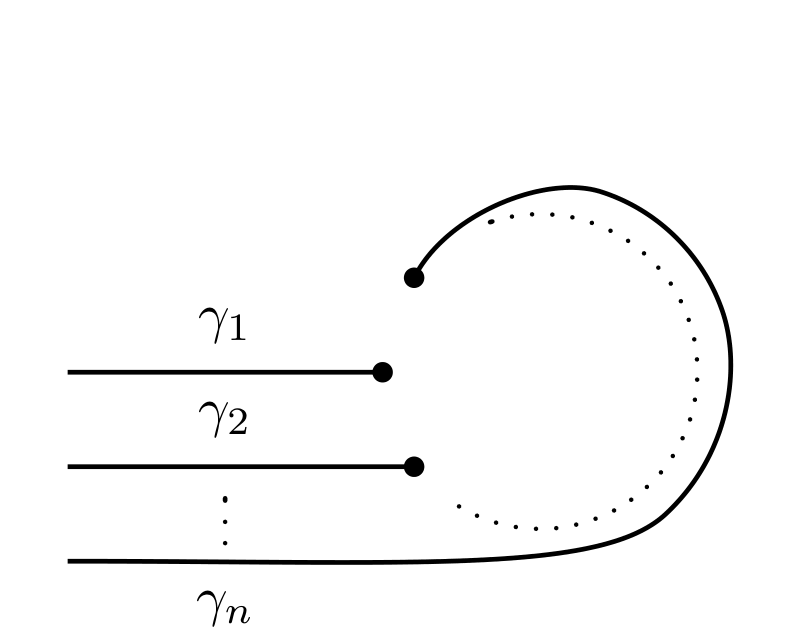
\includegraphics[width=\textwidth]{figures/fig13.1.png}
    \figtitle{13.1}{消没路径的临界集}
  \end{minipage}\hfill
  \begin{minipage}[b]{0.52\textwidth}
    \centering
    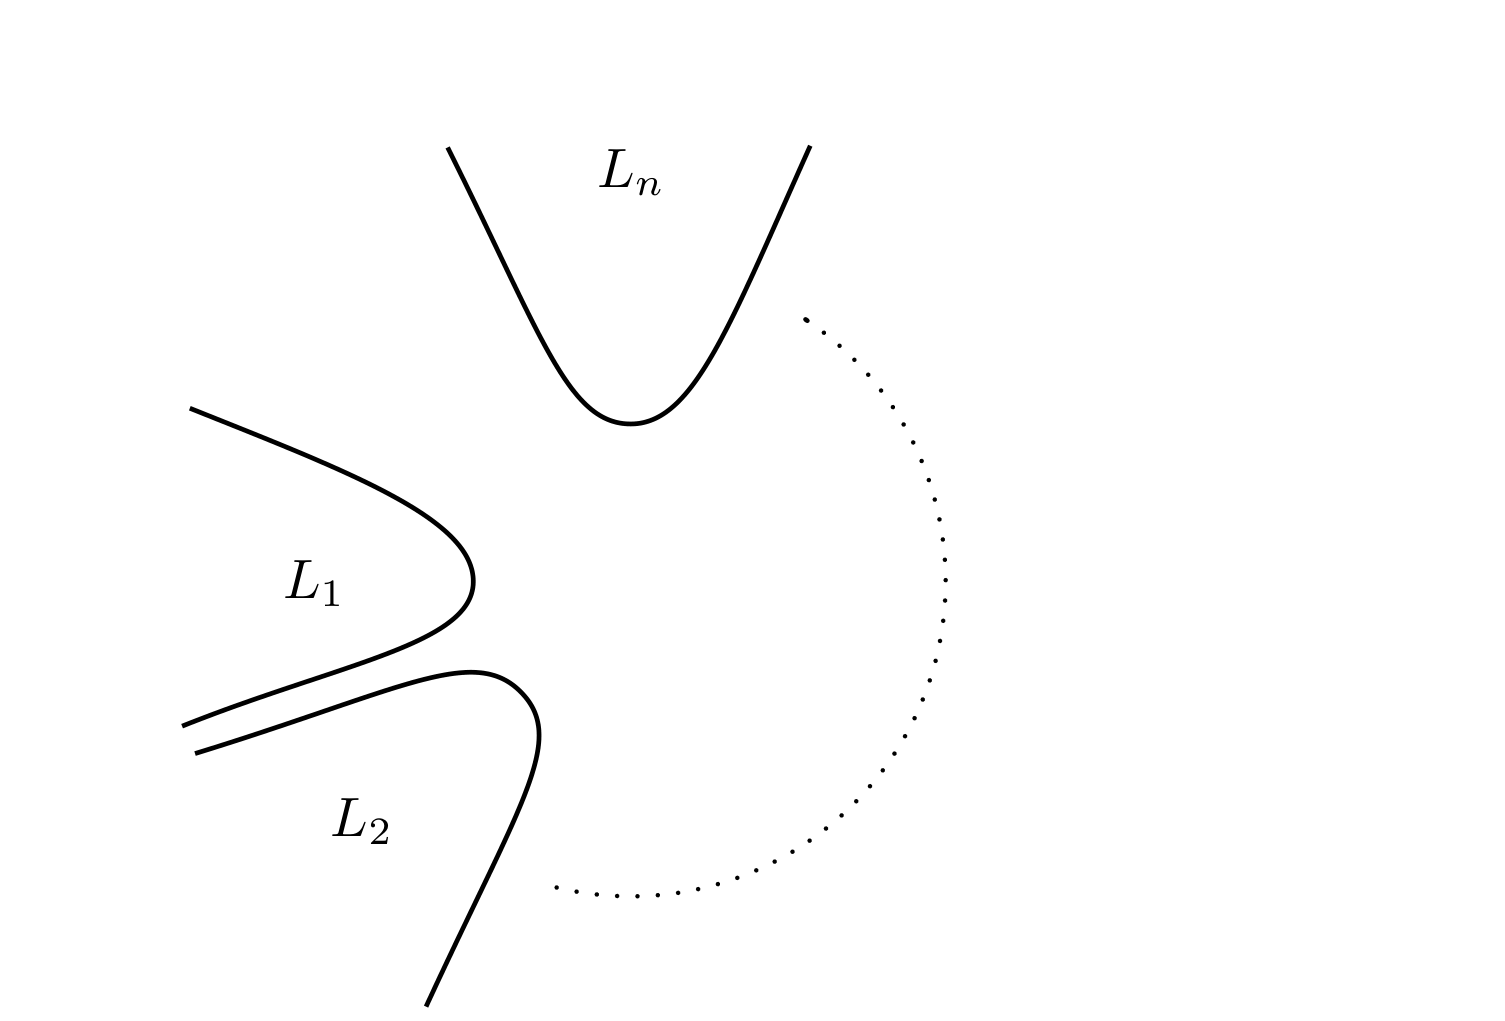
\includegraphics[width=\textwidth]{figures/fig13.2.png}
    \figtitle{13.2}{Lefschetz 穿透的特殊基}
  \end{minipage}
\end{figure}

\section{矩阵因子化}

对 Gorenstein 分次环\footnote{对 Abel 群 $H$，称给定了满足 $A_h\cdot A_{h'}\subset A_{h+h'}$ 的直和分解 $A=\bigoplus_{h\in H}A_h$ 的环为 $H$ 分次环（$H$-graded ring），或简称为分次环（graded ring）。对分次环而言，「所有素理想处的局部化都是 Gorenstein 局部环」与「所有齐次素理想处的局部化都是 Gorenstein 局部环」等价，满足这一条件的分次环称为 Gorenstein 分次环。} $R$，把有限生成分次 $R$-模构成的 Abel 范畴记为 $\mathrm{gr}\,R$，并把 $D^b\mathrm{gr}\,R$ 作为其有界导出范畴。$D^b\mathrm{gr}\,R$ 的对象若与投射模的有界复形拟同构，则称为完美复形（perfect complex）。把 $D^b\mathrm{gr}\,R$ 中由完美复形构成的满子范畴记作 $D^{\mathrm{perf}}\mathrm{gr}\,R$，称为完美导出范畴（perfect derived category）。有界导出范畴关于完美导出范畴的商\footnote{设 $\cT$ 为三角范畴，$\cN$ 为 $\cT$ 的满三角子范畴。把 $\cT$ 对使映射锥落入 $\cN$ 的态射集合进行局部化，便可再次得到三角范畴。称之为 $\cT$ 关于 $\cN$ 的 Verdier 商（Verdier quotient），记作 $\cT/\cN$。Keller [Dri04] 与 Drinfeld [Kel99] 证明了：增广三角范畴的 Verdier 商仍是增广三角范畴。} 称为稳定导出范畴（stable derived category）或奇点范畴（singularity category），并用
\begin{equation}
  D^b_{\mathrm{sing}}(\mathrm{gr}\,R) := D^b\mathrm{gr}\,R/D^{\mathrm{perf}}\mathrm{gr}\,R
  \tag{14.1}
\end{equation}
表示 [Buc87]。

% [Tutor Note: 原文脚注 54 的文献标记「Keller [Dri04] や Drinfeld [Kel99]」疑为张冠李戴
%  （[Dri04] 应为 Drinfeld、[Kel99] 应为 Keller）；此处按原文保留，请审校确认。]

正则分次环\footnote{对分次环而言，「所有素理想处的局部化都是正则局部环」与「所有齐次素理想处的局部化都是正则局部环」等价，满足这一条件的分次环称为正则分次环。} $S$ 与非零齐次元 $f\in S$ 给出的商环 $R:=S/(f)$ 是 Gorenstein 分次环的典型例子。此时稳定导出范畴可用 [Eis80] 引入的矩阵因子化（matrix factorization）具体描述\footnote{自由 $S$-模的无限序列 $K^{\bullet}=\left\{\cdots\to K^i\xrightarrow{k^i}K^{i+1}\xrightarrow{k^{i+1}}K^{i+2}\to\cdots\right\}$，若对任意 $i\in\Z$ 有 $K^{i+2}\cong K^i$ 且 $k^{i+1}\circ k^i=W$，则称为矩阵因子化（matrix factorization）。与复形的情形同样，矩阵因子化自然地构成微分分次范畴。关于矩阵因子化的解说，例如可参见 [Yos90]。}。

作为例子，考虑 $S:=\C[x]$、$f:=x^{n+1}$、$R:=S/(f)$ 的情形，则 $(E_i:=R/(x)(-i+1))_{i=1}^n$ 构成 $D^b_{\mathrm{sing}}(\mathrm{gr}\,R)$ 的完备例外序列，且它们之间的态射满足
\begin{equation}
  \Ext^k(E_i,E_j)\cong
  \begin{cases}
    \C\cdot\id_{S_i}, & i=j\ \text{且}\ k=0,\\
    \C, & j=i+1\ \text{且}\ k=1,\\
    0, & \text{其他}
  \end{cases}
  \tag{14.2}
\end{equation}
这一点容易看出 [Tak05, Orl09]。

% [Tutor Note: 原文 (14.2) 中的「id_{S_i}」疑为「id_{E_i}」之笔误（E_i 才是例外序列的元素），
%  此处按原文保留，请审校确认。]

\section{可逆多项式}

对以自然数为元素的 $n\times n$ 矩阵 $A$，定义 $n$ 元多项式 $f\in\C[x_1,\ldots,n]$ 为
\begin{equation}
  f=\sum_{i=1}^{n}x_1^{a_{i1}}\cdots x_n^{a_{in}}
  \tag{15.1}
\end{equation}
注意，$f$ 的非零系数可以通过把变量 $x_i$ 适当地乘以常数而规范化为 1。当 $A$ 为可逆矩阵、且 $f$ 在原点具有孤立临界点时，称 $f$ 为可逆多项式（invertible polynomial）。对 $f\in\C[x_1,\ldots,x_n]$ 与 $g\in\C[y_1,\ldots,y_m]$，称 $f+g\in\C[x_1,\ldots,x_n,y_1,\ldots,y_m]$ 为 $f$ 与 $g$ 的 Sebastiani–Thom 和（Sebastiani–Thom sum）[ST71]。一般而言，可逆多项式可由若干下述类型的 Sebastiani–Thom 和给出 [AGZV85, KS92]：

% [Tutor Note: 原文「C[x_1,\ldots,n]」中末项漏写了下标 x，应为 C[x_1,\ldots,x_n]；此处按原文保留，请审校确认。]

\begin{itemize}
  \item Fermat 型（Fermat type）：$f=x^p$
  \item 链型（chain type）：$f=x_1^{p_1}x_2+x_2^{p_2}x_3+\cdots+x_{n-1}^{p_{n-1}}x_n+x_n^{p_n}$
  \item 环型（loop type）：$f=x_1^{p_1}x_2+x_2^{p_2}x_3+\cdots+x_{n-1}^{p_{n-1}}x_n+x_n^{p_n}x_1$
\end{itemize}

对给定的可逆多项式，环 $\C[x_1,\ldots,x_n]/f$ 具有由 $(n+1)$ 个生成元 $\vec x_1,\ldots,\vec x_n,\vec c$ 与 $n$ 个关系式
\begin{equation}
  a_{i1}\vec x_1+\cdots+a_{in}\vec x_n=\vec c,\qquad i=1,\ldots,n
  \tag{15.2}
\end{equation}
定义的秩 1 的 Abel 群 $L$ 所给出的自然分次。这个 $L$ 是由
\begin{equation}
  K:=\left\{(\alpha_1,\ldots,\alpha_n)\in(\C^\times)^n\;\middle|\;
  \alpha_1^{a_{11}}\cdots\alpha_n^{a_{1n}}=\cdots=\alpha_1^{a_{n1}}\cdots\alpha_n^{a_{nn}}\right\}
  \tag{15.3}
\end{equation}
定义的群的特征标群。最大对角对称群（the group of maximal diagonal symmetries）$G_{\max}$ 定义为映射
\begin{equation}
  K\to\C^\times,\qquad (\alpha_1,\ldots,\alpha_n)\mapsto\alpha_1^{a_{11}}\cdots\alpha_n^{a_{1n}}
  \tag{15.4}
\end{equation}
的核：
\begin{equation}
  1\to G_{\max}\to K\to\C^\times\to1.
  \tag{15.5}
\end{equation}
(15.5) 诱导出特征标群的正合列
\begin{equation}
  0\to\Z\to L\to G_{\max}^{\vee}\to0
  \tag{15.6}
\end{equation}
这里，
\begin{equation}
  G_{\max}^{\vee}:=\Hom(G_{\max},\C^\times)
  \tag{15.7}
\end{equation}
与 $G_{\max}$ 之间有一个并非典范（canonical）的同构。把 $A$ 的逆矩阵置为
\begin{equation}
  A^{-1}=
  \begin{pmatrix}
    \varphi_1^{(1)} & \varphi_1^{(2)} & \cdots & \varphi_1^{(n)}\\
    \varphi_2^{(1)} & \varphi_2^{(2)} & \cdots & \varphi_2^{(n)}\\
    \vdots & \vdots & \ddots & \vdots\\
    \varphi_n^{(1)} & \varphi_n^{(2)} & \cdots & \varphi_n^{(n)}
  \end{pmatrix}
  \tag{15.8}
\end{equation}
则 $G_{\max}$ 由
\begin{equation}
  \rho_k:=\left(\exp\left(2\pi\sqrt{-1}\varphi_1^{(k)}\right),\ldots,
  \exp\left(2\pi\sqrt{-1}\varphi_n^{(k)}\right)\right)
  \tag{15.9}
\end{equation}
生成。对 $i=1,\ldots,n$ 置
\begin{equation}
  \varphi_i\colon\varphi_i^{(1)}+\cdots+\varphi_i^{(n)}
  \tag{15.10}
\end{equation}
并令群同态 $\varphi\colon\C^\times\to K$ 由
\begin{equation}
  \varphi(\alpha):=\left(\alpha^{\ell\varphi_1},\ldots,\alpha^{\ell\varphi_n}\right)
  \tag{15.11}
\end{equation}

% CHUNK c06 DONE pages p022–p023
